\documentclass[crop,tikz]{standalone}

\usepackage{pgfplots}
\tikzset{>=latex}
\colorlet{green}{black!40!green}

\pgfplotsset{
  inverted/.style = {
    every axis legend/.append style={
      draw=white,
      fill=hardblack,
      text=white
    }
  },
  every non boxed x axis/.append style={
    axis line style={-latex}
  },
  every non boxed y axis/.append style={
    axis line style={-latex}
  }
}

\begin{document}
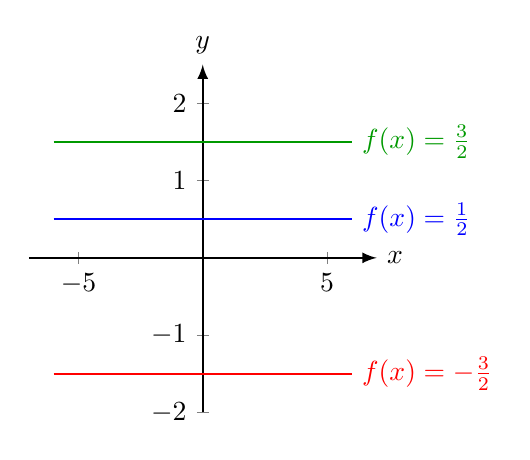
\begin{tikzpicture}
\begin{axis}[
  thick,
  width=6cm,
  height=6cm,
  xlabel={$x$},
  ylabel={$y$},
  xmin = -7, xmax = 7,
  ymin = -2, ymax = 2.5,
  axis y line=middle,
  axis x line=middle,
  xlabel style={at=(current axis.right of origin), anchor=west},
  ylabel style={at=(current axis.above origin), anchor=south},
  ytick distance=1,
  samples=10,
  domain=-6:6,
  smooth,
  clip=false,
  ]
  \addplot[red] {-1.5} node[right] {$f(x)=-\frac{3}{2}$};
  \addplot[blue] {0.5} node[right] {$f(x)=\frac{1}{2}$};
  \addplot[green] {1.5} node[right] {$f(x)=\frac{3}{2}$};
\end{axis}
\end{tikzpicture}
\end{document}
